% vim: set tw=78 sts=2 sw=2 ts=8 aw et ai:

The server is composed of multiple services that are all part of a process
running in a Java VM:

\begin{itemize}
  \item Android Proxy Service. This handles communication between the clients
        and the other services.
  \item Android Client Service. This keeps track of the trajectory and safety
        status of each mobile client over time.
  \item Safe Location Service. This is used to store information about exit
        points that is learned from the clients.
  \item Criteria Score Calculator and Spark Service. These are the modules
        involved in the computation of the optimal exit path requested by
        clients.
\end{itemize}

Communication with clients is done over TCP sockets, as JSON-formatted messages.
The following message types can be sent unidirectionally by the clients, and
no response is expected back from the server:

\begin{itemize}
  \item "client-location": A client can communicate its current position to
        the server, who will store it in the Android Client Service.
  \item "safe-location": Clients also have the ability to inform the server
        about exit points. In the current implementation this information is
        trusted blindly by the server, but future iterations should use
        techniques such as Bayesian inference to establish a degree of
        certainty about the actual safety of these locations. Note that
        upon receiving a new safe location, no action is taken by the server
        to inform the other connected clients about it, since this must be
        solicited explicitly.
  \item "friends": Clients can tell the server about other clients they wish
         to stay near to.
  \item "delete-clients" and "delete-safe-locations": These commands were used
        in the development phase of the application, in order to initiate the
        simulation of a new emergency event.
\end{itemize}

There is another category of client messages for which the server is expected
to send a response:

\begin{itemize}
  \item "safe-location-preferences": Should be sent at the beginning of the
        communication by the client, to inform the server of its preference
        for the 4 possible criteria: "safety", "proximity", "notCrowded" and
        "closeToFriends". A "consistency-ratio" response is expected from the
        server, informing the client whether the provided information make
        sense and can be used in the decision-making algorithm.
  \item "safe-location-request": This message triggers the decision making
        algorithm on the server, customized with the requesting client's
        information and preferences. A "safe-location-response" is issued on
        the way back, giving the latitude and longitude of the selected best
        exit point, along with its score in the decision algorithm.
\end{itemize}

The Multiple-Criteria Decision Analysis (MCDA) algorithm used is Analytic
Hierarchy Process (AHP).

\begin{figure}
\centering
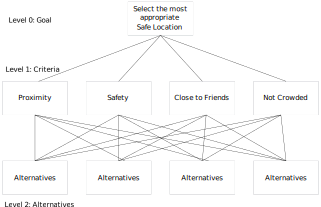
\includegraphics[scale=0.3]{ahp}
\caption{\label{fig:ahp} Analytic Hierarchy Process}
\end{figure}

